\subsection{Definition und Struktur}

Der Einfachheit halber wird in diesem Abschnitt der Raum $\mathbb{R}^2$ anstatt der unter~\ref{subsec:voronoi-introduction} eingeführte Raum $\mathbb{R}^m$ verwendet.

\subsubsection{Voronoi-Region}
Die Voronoi-Region $VR(p, O)$ besteht aus allen Punkten der Ebene, denen der Punkt $p = {p_x, p_y}$ näher ist als jeder andere Punkt aus der Punktemenge $O$.

\subsubsection{Voronoi-Diagramm}
Entfernt man nun sämtliche Voronoi-Regionen aus der Ebene, bleiben genau die Punkte des Raumes $\mathbb{R}^2$ übrig, die keinen eindeutigen sondern zwei oder mehr nächste Nachbarn in der Objekt-Menge $O$ besitzen.

Diese Punktemenge ist das \textit{Voronoi-Diagramm} $V(O)$ von $O$. \parencite{klein2005algorithmischegeometrie}

\begin{figure}[h]
\centering
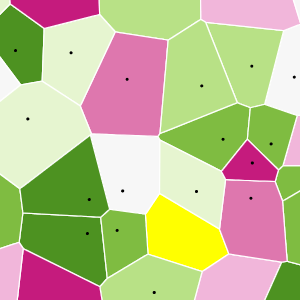
\includegraphics[width=150px]{images/voronoi_example_01.png}
\caption{Beispiel eines Voronoi-Diagramms}
\label{fig:voronoiExample01}
\end{figure}

\subsubsection{Voronoi-Kante und -Knoten}
Ein gemeinsames Randstück von zwei Voronoi-Regionen wird als \textit{Voronoi-Kante} bezeichnet, die Ecken einer Voronoi-Region werden als \textit{Voronoi-Knoten} bezeichnet.

\begin{figure}[h]
\centering
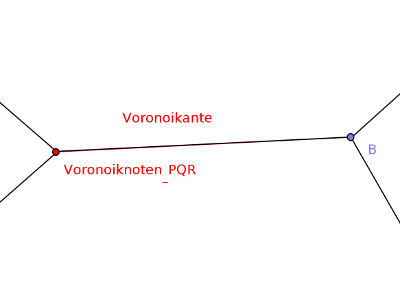
\includegraphics[width=150px]{images/voronoi_kante_knoten.png}
\caption{Beispiel einer Voronoi-Kante und eines Voronoi-Knotens}
\label{fig:voronoiExample01}
\end{figure}
